\documentclass[11pt]{article}
\RequirePackage{fullpage}
%\RequirePackage[font=small,labelfont=bf]{caption}
\RequirePackage{amsmath,amssymb,amsthm}
\RequirePackage{graphicx}
\RequirePackage[hidelinks]{hyperref}
\RequirePackage{subcaption}
\RequirePackage{wasysym}
\RequirePackage{authblk}
\RequirePackage{bm}
\RequirePackage{bbm}

\RequirePackage{cleveref}
\RequirePackage{xr}
\externaldocument{supplementary}

%\RequirePackage[osf]{mathpazo}
\let\temp\rmdefault
\RequirePackage{mathpazo}
\let\rmdefault\temp

\RequirePackage[bibstyle=authoryear,citestyle=authoryear-comp,
                date=year,
                maxbibnames=9,maxnames=5,maxcitenames=2,
                backend=biber,uniquelist=false,uniquename=false,
                % style=apa,
                sorting=nyt,
                % sorting=,
                hyperref=true]{biblatex}
\usepackage{color}
\usepackage{nicefrac}


% line numbers:
\RequirePackage{lineno}
%\modulolinenumbers[5]
\renewcommand\linenumberfont{\normalfont\tiny\sffamily\color{black}}

\renewcommand{\P}{\mathbb{P}}
\newcommand{\E}{\mathbb{E}}
\newcommand{\V}{\text{V}}
\DeclareMathOperator{\var}{var}
\DeclareMathOperator{\cov}{cov}

\addbibresource{biblio.bib}

%\title{Towards a Complete Model of the Negative Selection Process in Humans}
%\title{An Evolutionary Quantitative Genetic Model of the Negative Selection Process in Humans}
\title{A Quantitative Genetic Linked Selection Model fit to the Negative Selection Process in Humans}

\author{Vince Buffalo and Andrew Kern}

\begin{document}
\maketitle



\begin{abstract} 
% TODO: emphasize connection to nearly neutral theory
\end{abstract}


\section*{Introduction}

The continual influx of new mutations into populations is the ultimate source
of all adaptations, but the vast majority of mutations either do not affect
fitness or are deleterious. Negative selection (i.e. purifying selection) works
to eliminate such deleterious mutations from the population, which is essential
to maintaining the integrity of information in the genome needed to maintain a
lineage. Mutations under negative selection are kept at low frequencies
(Haldane?), contributing to human traits (XXX) and diseases. Moreover, the
negative selection process determines sequence conservation across phylogenetic
timescales, which is evident in genome-wide cross-species comparisons
\parencite{Siepel2005-wh}. As with most selection in the genome, the negative
selection process stochastically perturbs the allele frequencies of neighboring
linked variation. This reduces genetic variability to create a large-scale
spatial linked selection ``reduction signal" in genome-wide diversity. Mutation
and negative selection's contribution to this signal is mediated by the
deleterious mutation rate, the strength of selection in conserved segments, and
the spatial distribution of recombination rates and conserved segments. Since
genome-wide recombination maps and putatively conserved segments are available
for many species, researchers have combined these with population genetic
theory to estimate the mutation rate and selection coefficients of deleterious
mutations, as well as the overall reduction in genetic variability due to the
negative selection process.

Classic Background Selection (BGS) theory is the predominant theoretic model to
predict the reduction in linked neutral diversity, and is used by statistical
approaches that quantify the aspects of the negative selection. However, the
BGS model makes some assumptions for mathematical tractability that could
distort inferences about the negative selection process. First, since fixation
probabilities ultimately depend on the product of the deleterious selection
coefficient (s) and population size (N), the efficacy of negative selection
should depend on demography. Unfortunately, accommodating demography into
theoretic negative selection models remains an open, difficult problem (XXX).
Second, building off classic models of mutation-selection balance (Crow 1970,
Kimura and Maruyama 196), the Background Selection (XXX) model assumes that new
mutations are sufficiently deleterious that they are invariably driven to loss.
Under this assumption, the effect of selection is well-approximated by simply
rescaling the neutral coalescent by a reduction factor known as B (XXX).
However, this is only appropriate in a limited domain of parameters relevant to
the negative selection process (XXX). Because the BGS model cannot accommodate
the possibility of fixation for mutations with $Ns \ll 1$, diversity is
incorrectly predicted to fall to zero as the strength of selection diminishes.
This weak selection problem is related to the wider problem of modeling the
substitution rate of deleterious mutation (i.e. the “ratchet” rate). Third, the
BGS model assumes segments under purifying selection are sufficiently far apart
that there is no selective interference between them. This is a matter of
degree, since under sufficiently high mutation rates or with little
recombination, selective interference can occur with a segment. 

In this work, we extend another class of linked selection models that derive
from quantitative genetics to address limitations of classic background
selection theory. These models suggest that the reduction in pairwise
coalescence times at a position in the genome is determined by the
recombination map and distribution of polygenic additive fitness variance along
the chromosome \parencite{Santiago1998-bs}. This reduction is due to cumulative
effect of stochastic perturbations from selection at other sites. While these
models can theoretically accommodate polygenic fitness variation from any
source as long as its rate of change is not too rapid, we focus specifically on
a deleterious-mutations-only model from Santiago and Caballero (2016). This
model is identical to the classic BGS model when selection against deleterious
mutations is strong, but it also correctly predicts the reduction in diversity
and substitutions rates of weakly deleterious mutations by accurately modeling
levels of genic fitness variation. We extend Santiago and Caballero’s
(hereafter the SC16) model so that it can be used to model genome-wide patterns
of diversity under negative selection processes, and develop Python software to
use this theoretic approach to fit genome-wide models of negative selection.
Using forward simulations, we show this model leads to more accurate DFE
estimates under weak selection. While this new model accommodates the
possibility that a given reduction B could be due to weaker selection, in
applying our composite likelihood method to human population genomic data, we
confirm earlier findings that strong negative selection at a small fraction of
sites fits human data across populations best. Finally, we show that while this
model solves some limitations of the classic BGS model, simulations reveal
another mysterious defect: a poor fit around $Ns=1$. We show that this can be
partially corrected by incorporating the effects of selective interference on
genic variation, but the remaining discrepancy is due to the build up of
negative linkage disequilibrium that cannot be adequately captured by this
model. We find accounting for genic selective interference between segments
fits human population genomic data slightly better, suggesting levels of
negative selection in humans are sufficient to perturb the selection at other
sites.

\section*{Theory}

Our work is motivated by a well-known limitation of classic background
selection theory: it is only accurate for strongly deleterious mutations
\parencite{Charlesworth1993-gb,McVean2000-bt,Good2013-lp,Gordo2002-dr}. Given
statistical methods that fit linked selection processes to genome-wide
diversity data rely on the classic BGS model to estimate the distribution of
fitness effects and rate of deleterious mutations, it is important to
characterize and remedy these shortcomings. However, extending background
selection theory to model weak negative selection is challenging, and it is
worthwhile to develop some intuition for why this is the case, how the classic
background selection works, and how the quantitative genetic model of
\textcite{Santiago2016-mu} solves these problems and can be extended to
genome-wide inference.

Both the classic background selection and SC16 models imagine a negative
selection process where a continual influx of deleterious mutations flow into
the population at a rate of $\mu$ per basepair per generation in a conserved
region of $L$ basepairs, such that the region-wide per generation mutation rate
is $U = \mu L$. Each mutation imposes an additive selective cost of $s$ in
heterozygotes and $2s$ in homozygotes. The classic background selection model
only consider mutations that are sufficiently deleterious that they are
destined to extinction
\parencite{Charlesworth1993-gb,Nordborg1996-nq,Hudson1995-pt,Hudson1994-oh}. In
this case, the genealogy is well-approximated by a neutral coalescence process
with a rescaled effective population size of $N_0 = N \exp(-\nicefrac{U}{s})$.
This approximation works reasonably well for two reasons (though see
\cite{Cvijovic2018-vd,Walczak2012-fi,Nicolaisen2012-vs}). First, when selection
is strong, the number of deleterious mutations per haplotype has a stationary
Poisson distribution with an average equal to the equilibrium under the
deterministic mutation-selection model \parencite{Haldane1927-ga}. Since
lineages carrying strongly deleterious mutations cannot contribute to the
genealogy in the long run, coalescence events only occur in the fraction
$\exp(-\nicefrac{U}{s})$ of the population free of mutations. Second, the time
it takes for a present-day lineage to trace their ancestry back to a
mutation-free ancestor (the ``delay phase") is negligible compared to the
coalescence timescale of $N_0$ among these ancestors (the ``coalescence
phase"), and can be ignored (\cite{Durrett2008-ql}, p. 213;
\cite{Good2014-yz}).

When mutations are only weakly deleterious, their allele frequencies are
strongly influenced by stochastic perturbations and their frequency
trajectories are no longer well-approximated by deterministic models. When
genetic drift is the only source of randomness in allele frequency change, the
relevant scale of stochastic perturbations is determined by the drift-effective
population size $N_e$ (e.g. due to only non-selective process). The insight of
nearly neutral theory \parencite{Ohta1971-gq,Ohta1992-yi} is determined by the
compound parameter $2N_e s$. When $2N_e s \gg 1$, the stochastic component of
allele frequency change is minuscule relative to selection and can be ignored;
this is why the factor that rescales the drift-effective population size under
the BGS model does not depend on $N_e$. However, when $2N_e s \le 1$, the
stochastic perturbations are on a scale equal to or greater than the changes
due to selection. In this regime, weakly deleterious alleles can drift up to
intermediate frequencies before their eventual loss or fixation. When this
occurs, classic BGS theory breaks down for several reasons. First, the ``delay
phase" is no longer negligible as lineages carrying weakly deleterious
mutations can persist on coalescent timescales. This distorts genealogies away
those expected under neutrality
\parencite{Przeworski1999-mb,OFallon2010-my,Higgs1995-xc}. Second, the
distribution of the number of deleterious mutations (and its corresponding
fitness distribution) are no longer stationary and become a traveling wave
\parencite{Rouzine2008-qz,Good2013-lp,Gessler1995-hz} towards reduced
population fitness (since beneficial and back mutations are ignored).
Consequently, individuals in the least-loaded class are stochastically lost,
fixing those mutations with a click of ``Muller's ratchet"
\parencite{Muller1964-ki}. Determining both the rate of Muller's ratchet
\parencite{Haigh1978-gt,Gordo2002-dr,Gessler1995-hz} and the shape of
genealogies under weak selection have been stubborn open problems in
evolutionary genetics.

To further complicate matters, both strong and weakly deleterious mutations
create \emph{heritable} fitness variation. In turn, the presence of heritable
fitness variation generates another source of randomness in allele frequency
change known as genetic \emph{draft} \parencite{Neher2013-dz}. An allele
experiences genetic draft when it becomes randomly associated with a fitness
background, which stochastically perturbs its trajectory across generations.
Like genetic drift, perturbations due to draft are directionless but overall
increase the variance in allele frequency change. Unlike drift, stochastic
perturbations caused by draft are autocorrelated across generations for as long
an allele does not recombine or segregate off its fitness background and the
selective environment does not change
\parencite{Robertson1961-ho,Santiago1995-hx,Buffalo2019-qs}. When selection is
strong, draft can generate multiple-merger coalescences that create
discontinuities in allele frequency trajectories, making diffusion
approximations ill-suited \parencite{Gillespie2000-mh,Der2011-it,Neher2013-dz}.
However, when selection is weak, draft is well-approximated as an increase in
the rate of drift (or equivalently, a reduction in effective population size).

A key insight from Robertson (\citeyear{Robertson1961-ho}) is that in the
long-run weak draft acts like an increase in the variance in offspring number.
\textcite{Wright1938-tv} showed that additional non-heritable variance in
offspring number (e.g. due to mating strategy) rescales the population size
according to,

\begin{align}
    \label{eq:simple_Ne}
    N_e = \frac{2N}{V + 2}
\end{align}
%
where $V$ is the extra variance in offspring number.

However, unlike non-heritable variation in offspring number, the heritable
variation is autocorrelated across generations. At the individual level
Robertson considered, this is because offspring from large families tend to
beget many descendents themselves (and likewise with small families). The same
autocorrelation occurs at the genomic level, as the perturbations to a neutral
allele's trajectory from its particular fitness background tend to occur in the
same direction across generations as long as the linkage exists and the
selective environment is constant. Thus, the total additional heritable
variation in offspring number is the product of the equilibrium additive
fitness variation $V_A$ and an inflation factor $Q_t^2$ due to the build up of
autocorrelation to generation $t$. We let $Q^2 := Q_t^2$ as $t \to \infty$.
Intuitively, the product $V_A Q^2$ represents the expected total variance in
reproductive success a neutral mutation experiences over its lifetime in a
system with weak selection draft. Incorporating the impact of time-invariant
autocorrelation created by draft as a rescaled rate of drift is analogous to
using the Green--Kubo relation to find the transport coefficient in molecular
dynamics with velocity autocorrelation \parencite{Green1954-kl,Kubo1957-va}.

Including the total asymptotic variance in reproductive success in Equation
\eqref{eq:simple_Ne} and assuming Wright--Fisher levels of non-heritable
variation (i.e. $V = 2 + 4 Q^2 V_A$), the draft-effective population size $N_d$
is

\begin{align}
    \label{eq:main_Ne}
    N_d = \frac{N}{Q^2 V_A + 1}
\end{align}

(c.f. \cite{Robertson1961-ho,Santiago1995-hx}; see Supplementary Section
\ref{supp:theory} for a proof). In general, however, statistics such as
heterozygosity depend on the cumulative autocorrelation factor up to some time
$t$, $Q_t^2$ \parencite[p. 2111]{Santiago1998-bs}. This reflects the fact that
effective population size experienced by a mutation newly associated with a
fitness background is larger than the asymptotic effective population size,
since not much autocorrelation has accumulated in the stochastic perturbations
caused by drift yet. From a backwards-time perspective, this reflects the fact
that pairwise diversity (which is approximately heterozygosity when $2N\mu \ll
1$) depends on the pairwise coalescence rate per generation, which is not
constant under draft. The benefit of using Robertson's forward-time model of
draft is that the inflation factor is invariant with respect to the particular
fitness background the neutral allele becomes stochastically associated with.
By contrast, the difficulty with modeling draft backwards in time is that the
coalescence rates experienced by a lineage are not invariant to which lineage
was sampled due to its particular associated fitness background.

Equation \eqref{eq:main_Ne} is general, since different modes of selection and
linkage can be accommodated by different expressions for the inflation factor
$Q^2$ \parencite{Santiago1995-hx,Santiago1998-bs}. When fitness variation has a
multiplicative polygenic basis, as is often assumed for genome-wide negative
selection processes, the draft asymptotic effective population size experienced
by an arbitrary neutral site under the influence of all linked regions is,

\begin{align}
    \label{eq:polygenic_Ne}
    N_d \approx N \exp\left(-\sum_{i=1}^n V_{A,i} \frac{Q_i^2}{2}\right)
\end{align}

where the factor of one-half comes from ignoring weak associations from
unlinked regions and chromosomes (see Supplementary Section
\ref{supp:heritable-fitness}). In our genome-wide model, we consider the
summation in Equation \eqref{eq:polygenic_Ne} over non-overlapping segments $i
\in \{1, 2, \ldots, S\}$ each undergoing selection such that segment $i$
contributes additive fitness variance $V_{A,i}$ to the total additive genetic
fitness variance. Under equilibrium levels of fitness variation, the
autocorrelation function for a neutral allele associated with segment $i$ is
$C(t) = [(1-r_i)(1-\kappa_i)]^t$, where $r_i$ is the recombination fraction to
the segment and $\kappa_i$ is the rate that the associated fitness variance
decays due to selective dynamics. Then, the cumulative autocorrelation is,

\begin{align}
    \label{eq:Q}
    Q_i &= 1 + \sum_{j=1}^\infty \left[(1-r_i)(1-\kappa_i)\right]^j \nonumber \\
        &= \frac{1}{\kappa_i + r_i(1-\kappa_i)}.
\end{align}

(see Appendix Equation \ref{eq:Qinf}). This general equation can accommodate
models of polygenic selection as long as the equilibrium additive fitness
variation $V_{A,i}$ can be specified and the change in variance due to
selection can be approximated as a geometric decay, i.e. $\Delta V_{A,i} =
-\kappa V_{A,i}$ \parencite{Bulmer1971-ae,Keightley1988-eq,Walsh2018-bt}. This
is usually a reasonable assumption since within-generation selection removes a
fraction of phenotypic variation from the population, and some fraction of that
is additive genetic variation \parencite{Bulmer1971-ae,Keightley1988-eq}.

The remaining pieces are expressions for the equilibrium additive fitness
variance $V_A$ and the decay rate in associated fitness $1-\kappa$. At this
point, we diverge from Santiago and Caballero (\citeyear{Santiago1998-bs},
\citeyear{Santiago2016-mu}) to note that the additive fitness variation is the
sum of additive \emph{genic} fitness variance $V_a$ (i.e. due to allele
frequencies) and the fitness covariance due to linkage disequilibria between
selected sites ($\delta_{LD}$), $V_A = V_a + \delta_{LD}$. Considering only the
genic variation, at equilibrium $\Delta V_{a,i} = 0$; thus, the loss in genic
fitness each generation due to selective dynamics $-\kappa V_{A,i}$ must be
equal to the increase in fitness variation due to new mutations each generation
($V_m$) and changes in the LD term \parencite{Bulmer1971-ae}. Note that the
loss in genic fitness due to drift is not time-invariant due to the build up of
autocorrelation, and considered elsewhere in the derivation (see Supplementary
Materials Equation \ref{eq:vardecay}). Then, at equilibrium $\kappa_i =
\nicefrac{V_{m,i}}{V_{a,i}}$ (see Supplementary Materials Equation \ref{eq:Z}). 

Under any selection model, the genic fitness variance created by a new mutation
(at frequency $x=\nicefrac{1}{2N}$) is $2s^2 x(1-x) \approx \nicefrac{s^2}{N}$.
For the entire population of $2N$ chromosomes, the fresh variance from mutation
each generation in segment $i$ is $V_{m,i} \approx U_is^2$ where $U_i = 2\mu
L_i$ is the diploid mutation rate per generation within the segment. Under
mutation-selection balance assumed by BGS, an $L_i$-basepair segment has genic
variance $V_{a,i}^{BGS} \approx U_i s$ (see Supplementary Materials Equation
\ref{eq:va_bgs}) and thus $\kappa_i^{BGS} = s$. Substituting $V_{a,i}^{BGS}$
and $\kappa_i^{BGS}$ in Equation \eqref{eq:simple_Ne} and simplifying, we have

\begin{align}
    N_d = N \exp \left( - \sum_i^n \frac{\mu L_i}{s(1 + r_i(1-s)/s)^2} \right) 
\end{align}

which is identical to the genome-wide model of background selection used in
previous studies \parencite{McVicker2009-ax,Elyashiv2016-vt,Murphy2022-sj}.
Thus, the classic background selection model is a special case of the more
general theory of Santiago and Caballero (\citeyear{Santiago2016-mu}), which
they had shown previously (\citeyear{Santiago1998-bs}).

When selection is weak, however, the additive fitness variance under the
classic BGS model is no longer accurate. \textcite{Santiago2016-mu} suggested
that this is due to the loss of fitness variation that occurs when a
segregating site fixes and its heterozygosity becomes zero. If we let $R$
represent the fixation rate (i.e. ratchet rate) in the region per generation,
each fixation removes the equivalent amount of equilibrium variation put in by
mutation. Thus, the steady-state genic variance under mutation and negative
selection is (omitting the segment index $i$ for clarity),

\begin{align}
  \label{eq:Va}
  V_{a} = (U - 2 R)s. 
\end{align}

where the condition $V_a \ge 0$ is met when the probability of fixation is less
than or equal to the neutral fixation probability of $\nicefrac{1}{2N}$, which
is held when considering deleterious mutations. This equation connects the
equilibrium additive genic fitness variance to the flux of new variation in due
to new deleterious mutations and the flux out due to their substitution and the
decline in mean population fitness. When $R=0$, selection is so strong it
cannot fix, and the equilibrium fitness variation is due entirely to young rare
mutations before their extinction $V_a = V_a^{BGS} \approx Us$. Santiago and
Caballero derive Equation \eqref{eq:Va} through Fisher's Fundamental Theorem of
Natural Selection, but we find an alternative proof (\cite{Higgs1995-xc}; see
Supplementary Materials Section \ref{supp:weak-strong}). We also find that the
steady-state additive genic variance in Equation \eqref{eq:Va} results from
diffusion models with a flux of mutations into discrete sites
(\cite{Kimura1969-jw}). 

%Our results differ from \parencite{Santiago2016-mu}, since we find from
%simulations their expression models the additive \emph{genic} fitness
%variation, not additive genetic fitness variation (see Section XXX). This is
%because Equation \eqref{eq:Va} does not capture the expected build-up of
%negative linkage disequilibria when selection is mildly deleterious.

While using Equation \eqref{eq:Va} in Equation \eqref{eq:main_Ne} leads to a
prediction for the draft-effective population size $N_d$, closed-form
expressions for the rate of the ratchet $R$ have generally been hard to find
\parencite{Haigh1978-gt,Higgs1995-xc,Gessler1995-hz}. The key insight of
\textcite{Santiago2016-mu} is that the ratchet rate under draft is determined
by the probability of fixation $p_F(N_d, s)$
\parencite{Kimura1962-su,Malecot1948-zv} using the draft-rescaled effective
population size, i.e. $R = N U p_F(N_d, s)$. Given this equation for the
ratchet and Equation \eqref{eq:polygenic_Ne} for $N_d$ under draft, we have a
system of two non-linear equations that can be solved numerically for $N_d$ and
$R$ for each segment,

\begin{align}
  \label{eq:main_eqns}
  N_d &= N \exp \left( -V_a \frac{Q^2}{2} \right) & \text{\emph{draft-effective population equation}} \\
  R &= \frac{4N_d U s}{\exp(4 N_d s)-1}  & \text{\emph{ratchet equation}}
\end{align}

where $V_a = (U-R)s$ as in Equation \eqref{eq:Va}. We denote the solutions to
these equation, which represent equilibria under mutation-selection-drift-draft
process, as $\widetilde{N}_d$ and $\widetilde{R}$. These equilibria also imply
an equilibrium level of additive fitness variation $\widetilde{V}_a$ in the
segment, are used to calculate the reduction at an arbitrary position in the
genome (see Methods 

With the equilibrium $V_a$ calculated at each segment for a particular $\mu$
and $s$, we can estimate the reduction factor $B(x) = \nicefrac{N_d}{N}$ at any
genomic position $x$ (see Methods XXX).

\section*{Results: Confirmation of Theory}

Similar to previous work, our method characterizes the negative selection
process through the signal left on nucleotide diversity at linked sites.
Although nucleotide diversity is a less-informative statistic than the full
site frequency spectrum, it is much easier to derive models of how selection
alters expected pairwise coalescence times at linked sites than to describe the
entire genealogy. Spatial patterns of pairwise diversity are highly variable
across eukaryotic genomes, as linked selection leads diversity to become
correlated with spatial heterogeneity in recombination rates and the density of
conserved sites. Statistical methods then fit observed diversity to the
expected level under a particular theoretic model of linked selection
processes. Consequently, statistical inferences about selection may be
incorrect when the underlying theory inaccurately predicts average pairwise
coalescence times.

\subsection*{Simulations of a Segment under Negative Selection}

\begin{figure}[htbp] \centering
    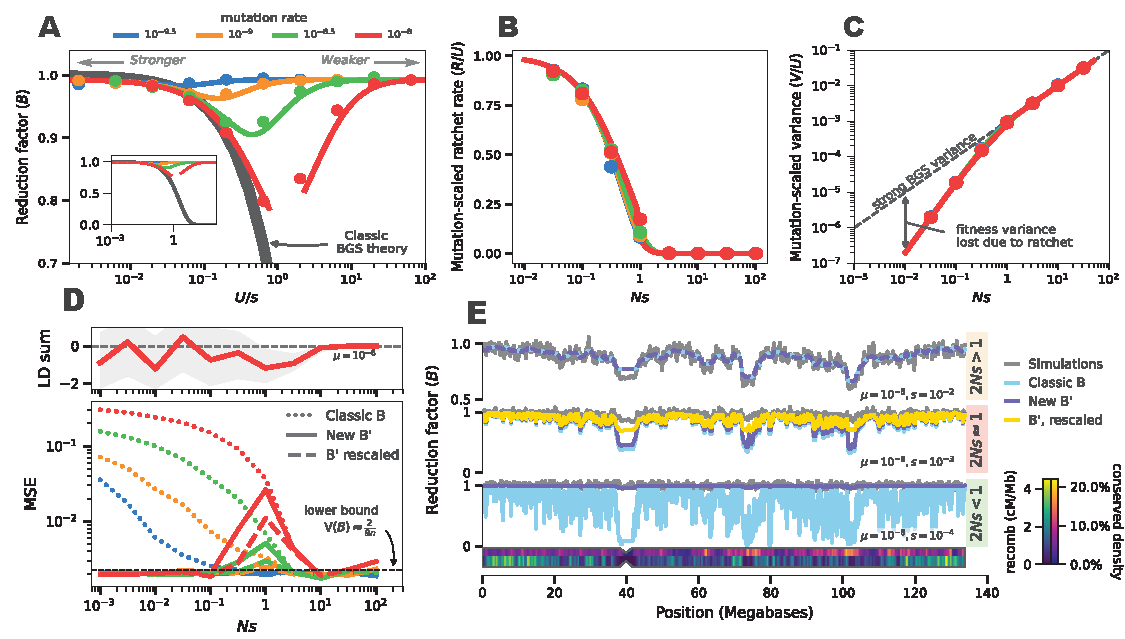
\includegraphics[width=\textwidth]{figures/figure_1.pdf} \caption{Theory
        compared to simulation results. (A) The predicted reduction factor
        under classic B theory (dark gray line) and the diploid SC16 model
        (colored lines corresponding to mutation rate) compared to average
        reduction across XXX simulation replicates (points). (B) The predicted
        ratchet rate under the SC16 model scaled by mutation rate (colored
        lines) compared to the ratchet estimated from simulation (points). When
        $2Ns>1$, the ratchet rate is near zero. (C) The genic variance from
        simulations (points) against the predicted variance under the SC16
        model (colored lines). As the ratchet begins to click, the genic
        variance is decreased from the level expected under strong BGS (dashed
        line). (D, bottom) The mean squared error (MSE) between
        whole-chromosome simulations and predicted classic B (dots), new B'
        (solid), and locally-rescaled B' (dashed) for different mutation rates
        (colors). The dashed horizontal line is the approximate theoretic
        minimum MSE. (D, top) The build up of negative linkage disequilibria
        around $2Ns=1$ in whole-chromosome simulations in bottom panel. (E) The
        average B map from 100 chromosome 10 simulation replicates (gray)
    against different predictions, for parameters that correspond to $2Ns < 1$,
$2Ns = 1$, and $2Ns > 1$. The chromosome shows the density of conserved sites
and recombination map used in simulations. }
  \label{fig:figure-1}
\end{figure}

Given that Santiago and Caballero's (\citeyear{Santiago2016-mu}) model is a
haploid-model for a single region under equilibrium negative selection, we
first sought to confirm it could accurately predict the reduction in realistic
forward-time simulations of diploid populations with recombination. Using SLiM
\parencite{Haller2019-vu,Haller2023-uk} we simulated a region of $10^5$
basepairs under varying levels of mutation and selection (see Methods
\ref{sec:methods-sim}). We find a close correspondence between the observed
and predicted reductions in effective population size $B=\nicefrac{N_d}{N}$
over all selection and mutation parameters including weak selection (Figure
\ref{fig:figure-1}A), in contrast to classic BGS theory. Furthermore, to
investigate whether this accuracy was caused by the model correctly predicting
the equilibrium fitness variance and ratchet rate, we also measured these
throughout the simulation. Again, we find the diploid SC16 theory accurately
predicts both the ratchet rate (Figure 1\ref{fig:figure-1}B) and the genic
fitness variance (Figure 1\ref{fig:figure-1}C).

Moreover, these simulations provide intuition about the underlying negative
selection process. When mutations are strongly deleterious, there is no chance
they can fix, and the ratchet rate is zero (Figure \ref{fig:figure-1}B for $2Ns
> 1$). In this strong selection regime, the additive genic fitness variation
closely matches the theoretic deterministic equilibrium of $V_a = Us$ (dashed
gray line, Figure \ref{fig:figure-1}C) However, around $2N_e s \approx 1$, the
ratchet begins clicking as $p_F > 0$. When this occurs, each click of the
ratchet eliminates variation, and the equilibrium variation diverges from the
deterministic mutation-selection equilibrium (Figure \ref{fig:figure-1}C).

\subsection*{Chromosome-wide Simulations and Models of Negative Selection}

Given the accuracy of the SC16 model in predicting the reduction factor $B$ and
ratchet rate for a single segment under general mutation-selection processes,
we extended their model so that it could be applied to whole-genome data. Our
software method \texttt{bgspy} numerically solves Equations XXX to compute the
equilibrium additive genic fitness variance ($V_a$) and ratchet rate ($R$)
across grids of mutation rates and selection coefficients. This is done for
each pre-specified segment in the genome that may be under negative selection
(e.g. coding sequences or UTRs). Then, these equilibrium can be used to
calculate a reduction map $B(x)$ across genomic positions $x$. To distinguish
between McVicker's B maps based on classic BGS theory, we call our reduction
map $B(x)$ a B' map.

To assess our predicted B' reduction maps, we simulated negative selection for
fixed mutation rates and selection coefficient on human chromosome 10 using
realistic recombination maps and conserved feature positions. Averaging over
$100$ replicates, we estimated the simulation expected reduction map and
compared this to the predicted B and B' maps for the same parameters. We find
that our B' maps and the classic BGS theory B maps closely match simulations
when selection is strong (top row of Figure \ref{fig:figure-1}E). This provides
the first realistic forward-time chromosome-scale simulation confirmation of
classic BGS theory. However, we find slight discrepancies in regions with low
recombination (Figure \ref{fig:figure-1}E). Second, we find our theory is
vastly more accurate than the classic B maps when selection is very weak ($2N_e
s \ll 1$; bottom row of Figure \ref{fig:figure-1}E), which is expected since
BGS theory does not work in this domain. Across all mutation and selection
parameters simulated, the relative error of the classic B maps is 14.6\%
whereas the relative error in the new B' maps is 5\%. Additionally, we find
that the mean squared error between simulations and B' maps is close to the
theoretic lower bound set by the coalescence variance \parencite[see Methods
XXX]{Tajima1983-gu}.

Nearly all of the error between the new B' maps and chromosome-wide simulations
occurs around the drift-barrier domain of $2Ns \approx 1$ (Figure
\ref{fig:figure-1}D). The higher error in this domain occurs across all
mutation rates. We hypothesized that the higher error in this domain may be
because when our method numerically solves Equations \eqref{eq:main_eqns} for
each segment, it does not consider the reduction experienced due to selection
at other linked segments. In particular, we use a fixed drift-effective
$N=1000$ corresponding to the number of diploids in the simulations rather than
$B(x) N$ at position $x$. To test this, we implemented a locally-rescaled
version of the B' maps, which numerically solves Equations \eqref{eq:main_eqns}
for each segment at position $x$ taking into account the reduction experienced
due to selection at other segments by setting $B'(x)N$ as the population size
(see Method XXX). We find the locally-rescaled B' maps reduce the relative
error from 5\% to 0.4\% and mean squared error (Figure \ref{fig:figure-1}D,
dashed colored lines), but does not entirely eliminate the error in the $2Ns
\approx 1$ domain. Overall, while we find evidence that local-rescaling
slightly reduces error in the $2Ns \approx 1$ domain, we do not use it during
in our genome-wide inference method. This is because to avoid circularity and
possible overfitting, the method would need to solve the equilibria equations
for all segments simultaneously, but this is currently computational
unfeasible.

Finally, we hypothesized that the remaining error is because of the build up of
negative linkage disequilibria between selected sites due to Hill--Robertson
interference \parencite{Hill1966-kd,McVean2000-bt,Comeron2007-wq}. To assess
this possibility, we calculated the sum of all linkage disequilibria in our
chromosome-wide simulations. We find negative linkage disequilibria build ups
around $2Ns \approx 1$ (Figure \ref{fig:figure-1}D, top row) and is stronger
when mutation rates are higher. As $Ns \to 0$, the variance in LD inflates as
expected \parencite{Ohta1969-ae,Hill1968-ue}. Overall, the build up of negative
LD is consistent our view that the equilibrium fitness variance modeled by the
SC16 theory is the additive \emph{genic} fitness variance, which differs from
the additive genetic variance by the sum of linkage disequilibria between
selected sites (i.e. $\delta_{LD} = s^2 \sum_{i\ne j} D_{i,j}$ where $D_{i,j}$
is the LD between sites $i$ and $j$). However, according to theory, the
reductions in diversity should be determined by levels of additive genetic
fitness variance that include the contribution of LD (Supplementary Materials
Section \ref{supp:theory}).

\section*{Results: Application to Human Genomic Data}

\subsection*{Annotation Model Comparison}

Our composite likelihood method takes tracks of annotated features (an
``annotation model") that are \emph{a priori} expected to have similar fitness
effects, and estimates the overall mutation rate and distribution of fitness
effects for each feature type. We consider two classes of annotation models:
(1) CADD-based models, which consider the top $x\%$ of basepairs according to
the CADD pathogenicity score assigned to each basepair, and (2) and more
interpretable gene feature-based models that includes protein coding regions,
intron and UTRs, and PhastCons regions. We include PhastCons regions because
there is strong evidence of highly-conserved non-coding regions
\parencite{Meader2010-hm,Harmston2013-tt,Katzman2007-gq,Siepel2005-wh}, that
would be missed by gene feature only annotation. These two classes of
annotation models have a trade-off between fine-scaled specificity to which
basepairs are likely to be under negative selection, and interpretability of
the DFE estimates for each feature.

Our method estimates the distribution of fitness effects (DFE) for each feature
class. While CADD-based models only have a single conserved feature class (e.g.
CADD 6\%), feature-based models can have multiple feature classes under varying
levels of selective constrain. However, overlapping features (e.g. a basepair
that is annotated as both PhastCons and coding sequence) must be assigned to
one category or the other. Since this assignment impact DFE estimates, we fit
both of the two alternatives. First, a \emph{PhastCons Priority} model, where
genic features that overlap PhastCons regions are classified as PhastCons, and
all remaining coding basepairs are labeled as CDS. Second, a \emph{Feature
Priority} model, where all coding basepairs are assigned to CDS, and the
PhastCons class catches the remaining highly-conserved non-genic regions. 

In total, we fit four annotation models (CADD 6\%, CADD 8\%, PhastCons
Priority, and Feature Priority) to high-coverage 1000 Genome data for three
populations: Yoruba (YRI), Han Chinese (CHB), and European (CEU) reference
samples. We assess and compare our models according to how well they predict
patterns of diversity on whole chromosomes left-out during the model fitting
process (e.g. leave-one-chromosome-out, LOCO). We use the metric
$R_\text{LOCO}^2$, which is the proportion of the observed variance in genomic
diversity at the megabase scale predicted by our model. We experimented with a
few smaller spatial scales (e.g. 100 kbp), but our results were consistent with
previous results suggesting the human linked selection signal fits best at the
megabase scale \parencite{Murphy2022-sj}.

\begin{figure}[htbp] \centering
    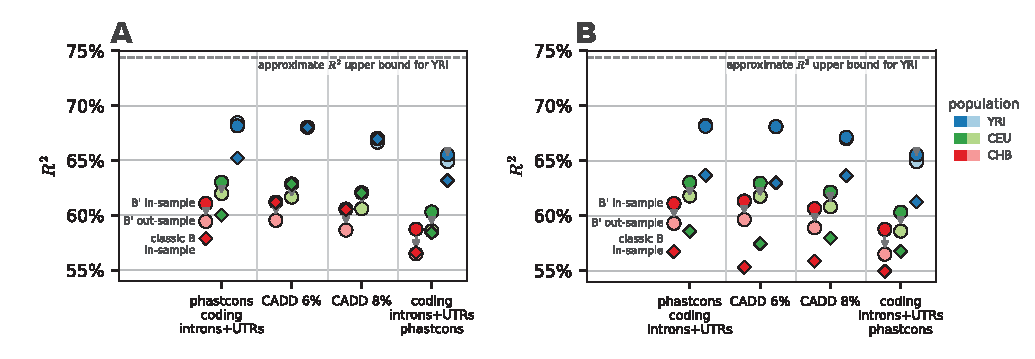
\includegraphics[width=\textwidth]{figures/figure_2.pdf} 
    \caption{The $R^2$ estimates for a sparse (A) and full (B) models, for all 
    populations (colors) fit at the megabase-scale. Round points are our B' 
    method and diamonds are the classic B. Lighter color round points are
    the out-sample $R_\text{LOCO}^2$ estimates for our B' method, and arrows show the decline
    in goodness-of-fit due to in-sample overfitting (out-sample $R_\text{LOCO}^2$ 
    were not calculated for classic B values due to computational costs). The 
    horizontal dashed lines are the $R_\text{drift}^2$ expected when the residual
    variance is given by the theoretic variance in coalescence times due to drift alone.}
  \label{fig:figure-2}
\end{figure}

Overall, we find the PhastCons Priority and CADD 6\% models fit about equally
as well (Figure \ref{fig:figure-2}A), consistent with recent work using classic
BGS theory \parencite{Murphy2022-sj}. However, we find that our models predict
out-sample diversity levels slightly better than previous methods. For these
two models, we find that our B' method predicts $R_\text{LOCO}^2=68.45$\% and
$R_\text{LOCO}^2=68.04$\% of the out-sample variance in Yoruba pairwise
diversity at the megabase-scale, respectively. By contrast, the best-fitting
CADD 6\% model from \textcite{Murphy2022-sj} explained 60\% of diversity in
left-out 2 Mbp windows across YRI samples. We note that this might be explained
by other differences in data process, reference genome, etc.

In populations impacted by the out-of-Africa bottleneck, the goodness-of-fit
was lower across all models (e.g. 62.98\% and 59.98\% for CEU and CHB
respectively in the PhastCons Priority model). Our PhastCons Priority model
fits marginally better than the CADD 6\% model consistently across all three
populations (Supplementary Table \ref{supp:tbl-r2}). This is likely because the
PhastCons Priority model has more DFE parameters, and thus can fit finer-scale
differences among the four feature types. By contrast, the CADD 6\% track must
fit patterns of diversity to conserved sites under a single DFE. The CADD 8\%
model fit slightly worse than the CADD 6\% across all populations, and the
Feature Priority model had the poorest-fit.

Since our method is built upon theory that fixes the weak selection problem of
classic BGS theory, it should in principle fit equally well when an annotation
model includes regions that are under no selective constraint and thus
neutrally evolving. To test this, for each of our annotation models (which are
``sparse") we fit a corresponding ``full" model that assigns the remaining
complement of the genome to a feature called ``other" that contains most of the
genome. Ideally, how a model fits using our B' method should be invariant to
whether an annotation model is sparse or full, since our method in principle
can accommodate weak selection and neutrality. Indeed, we find this to be the
case: both in-sample $R^2$ and out-sample $R_\text{LOCO}^2$ values are nearly
identical across full and sparse-track models (Figures \ref{fig:figure-2}A and
\ref{fig:figure-2}B, round points). 

By contrast, full annotation models fit poorly under classic BGS theory (Figure
\ref{fig:figure-2}B, diamond-shaped points) and lead to unreasonable parameter
estimates (discussed in Section XXX). Additionally, when sparse annotation
models contain genomic features that are likely under weak constraint (such as
introns and UTRs), models fit worse under classic BGS theory than our B' method
(Figure \ref{fig:figure-2}A). However, among the CADD annotation models, the
goodness-of-fit is nearly identical between B' and classic BGS methods. This
behavior is what we would expect given that the CADD models contain only the
most pathogenic sites, which are \emph{a priori} very likely under the strong
selection domain under which B' and classic BGS theory agree.

Overall, our $R_\text{LOCO}^2$ estimates suggest our negative selection model
explains up to 68\% of out-sample variance in diversity of the megabase scale,
even though our method assumes constant demography and homogeneous mutation
rates along the genome. A worthwhile question is: how much variation
\emph{could} we expect to fit at this scale? Given that selection alters
genealogies in ways beyond just decreasing mean pairwise coalescence time and
populations have non-constant demography, an exact analytic answer is
intractable. However, we can get an approximate idea if we assume that the
residual variance $\sum_b (\pi_b - \widehat{\pi}_b)^2$ is determined entirely
by the expected neutral coalescence noise around the expected coalescence time
$2B(b)N$. This can be be found analytically, plugging-in our predictions for
$B(b)$. This allows us to calculate $R_\text{coal}^2$ to ballpark the theoretic
variance that is capable of being explained, assuming this coalescence-only
noise process (see Method XXX). We note that selection is expected to
\emph{decrease} the variance in coalescence times beyond a rescaled effective
population size implies; our $R_\text{coal}^2$ would be an underestimate under
selection.

We find that our out-sample $R_\text{LOCO}^2$ for the Yoruba samples
($R_\text{LOCO}^2 \approx 68$\%) is slightly above the theoretic
$R_\text{coal}^2 \approx 67$\%. This suggests our model is close to the
vicinity of fitting all the signal possible, under the coalescence-only noise
assumption. By contrast, for bottlenecked out-of-Africa populations, we find a
larger discrepancy between $R_\text{coal}^2$ and observed out-sample
$R_\text{LOCO}^2$. The theoretic $R_\text{coal}^2 \approx 64$\% for both
populations, compared to the observed $R_\text{LOCO}^2 \approx 62$\% for CEU
and $R_\text{LOCO}^2 \approx 59$\% for CHB. Given that bottlenecks would act to
increase the residual variance in coalescence times beyond the level implied by
the effective population size, the gap would likely shrink under more realistic
models or simulation-based approximations for $R_\text{coal}^2$. Overall, this
suggests that negative selection models explain the vast majority coalescence
time variation at the megabase-scale that is capable of being explained (i.e.
that is not coalescence noise).

\subsection*{Estimated Distribution of Fitness Effects}

\begin{figure}[htbp] \centering
    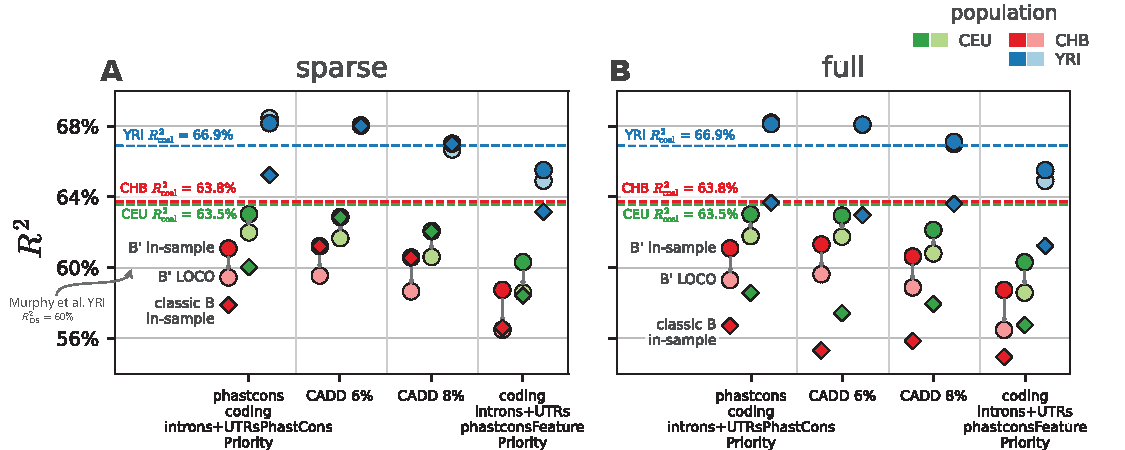
\includegraphics[width=\textwidth]{figures/figure_3.pdf} 
    \caption{The distribution of fitness effects of new mutations estimates for
        Yoruba individuals. (A) The DFEs using sparse (left column) and
        full-coverage (right column) tracks, across different annotation models
        (row). Color indicates the feature type. (B) The DFE of the
        full-coverage CDS-priority model comparing the estimates across
    populations.}
  \label{fig:figure-3}
\end{figure}

Our composite likelihood method has three sets of parameters: expected
diversity in the absence of linked selection diversity $\pi_0$, the mutation
rate $\mu$, and the distribution of fitness effects $\mathbf{W}$ across the
selection grid for each of the $K$ feature types. Given that the relationship
between $\pi$ and the strength selection is U-shaped, our model in theory could
fit under different combinations of parameters.

However, across all of our annotation models, new deleterious mutations in
conserved feature classes were consistently estimated to have strongly
deleterious effects (Figure \ref{fig:figure-3}A), consistent with previous work
\parencite{McVicker2009-ax,Murphy2022-sj}. This includes features such as
coding sequences, PhastCons regions, or the top 6\% of basepairs with the most
pathogenic CADD scores. However, we find that there is considerable uncertainty
in how strong selection is against the most deleterious mutations. For example,
in the CADD 6\% full-track model, new mutations are estimated to have a
selection coefficients of $s = 10^{-1}$ with 42\% chance, $s=10^{-2}$ with
7.8\% chance, and $s=10^{-3}$ with 41\% chance. This creates a bimodal DFE
(Figure \ref{fig:figure-3}A, second row, left column), which is mirrored across
the other CADD models. Moreover, these DFE estimates suggest a very high
average selection coefficient across CADD 6\% regions of $\widehat{\bar{s}}
\approx 0.043$ for YRI.

Given that previous methods have typically not estimated the DFE up to
selection coefficients of $s=10^{-1}$, we ran additional ``constrained grid"
models using a DFE only up to $s=10^{-2}$. Across all populations, these
constrained grid models fit the data less well than the default grid by about
one percentage point less in $R_\text{LOCO}^2$ (see Supplementary Table
\ref{supp:tbl-r2}). As expected, the constrained grid models distributed mass
onto the next strongest selection coefficient, $s=10^{-2}$, and the average
selection was reduced about six-fold to $\widehat{\bar{s}} \approx 0.0079$ for
YRI. While the DFE may truly be bimodal for highly-conserved regions and have a
very high average selection coefficient, a likely alternative is that these
results reflect a non-identifiability issue between selective effects of
$s=10^{-1}$ and $s=10^{-2}$. We will refer to this as the
\emph{strong-selection non-identifiability} issue.

We propose that one mechanism for this non-identifiability is that mutations
extremely harmful to fitness are difficult to distinguish from a smaller
effective population. Intuitively, as $s$ increases, the average persistence
time (in generations) of the mutation in the population goes below one
generation, i.e. death of the carrier of the \emph{de novo} mutation. In this
hypothetical limit, each occurrence of a very harmful mutation nearly acts like
an instantaneous death that in effect is just a smaller population size. One
way to test this hypothesis is to look to see if there is a systematic positive
relationship across models between average selection coefficient and $\pi_0$,
which is includes the drift-effective population size $N_e$.

We find this is the case for all of our CADD 6\% models. Across every
population, average selection was about $7.1$ times larger using the default
grid, and $\pi_0$ was $5.6\%$ larger. There was no similar consistent change in
mutation rate estimates among populations. In the CADD 6\% model, genome-wide
average reduction factor $\bar{B}$ was $\approx 6.1\%$ lower in the default
versus constrained grid. Overall, this suggests that the linked selection
signal alone cannot differentiate very strong selection from a slightly smaller
drift-effective population size.

Despite the strong-selection non-identifiability issue, we were curious how
stable these estimates are across different reference populations. Overall, the
DFE estimates were consistent over all populations and models (Supplementary
Materials Section \ref{supp:fits}). Here, we highlight the Feature Priority
model since though it is poor-fitting, the DFE estimates are more readily
interpretable since it is based on gene features. Figure \ref{fig:figure-3}B
shows consistent DFE estimates across populations, with narrow uncertainty as
estimated by a block jackknife procedure. Coding sequences have a bimodal DFE
consistent with the strong-selection non-identifiability issue. Additionally,
coding sequences have a very uncertain neutral mode in the DFE. This is
expected given the different level of selective constraint between synonymous
and non-synonymous sites. 

Additionally, the PhastCons class of this Feature Priority model, which
contains highly conserved non-coding elements, is under strong selective
constraint as expected. Finally, we highlight one result from our PhastCons
Priority annotation model (Figure \ref{fig:figure-3}A bottom row): the DFE
estimate for coding sequences excluding PhastCons regions is estimated as
neutral. This too is expected; the selection signal in coding regions is
absorbed by the PhastCons feature, leaving only conditionally neutral sites.

\subsection*{Estimates of the Deleterious Mutation Rate in Humans}

\begin{figure}[htbp] 
    \centering
    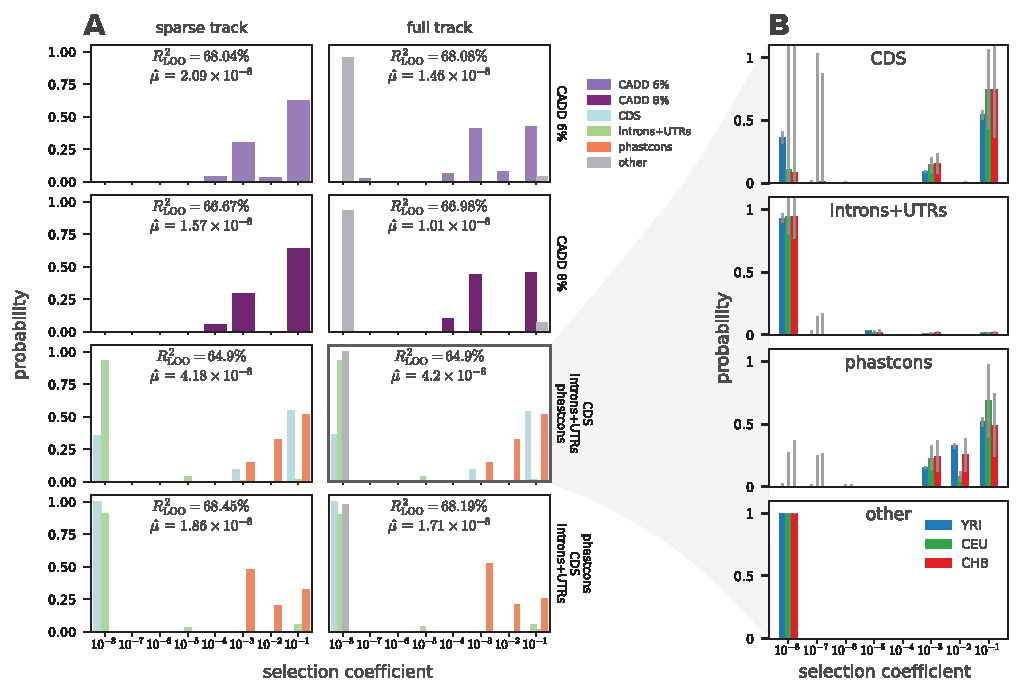
\includegraphics[width=\textwidth]{figures/figure_4.pdf} 
    \caption{(A) }
  \label{fig:figure-4}
\end{figure}

Early genome-wide classic BGS models fit well, but lead to unusually high
estimates of the mutation rate \parencite{McVicker2009-ax}. This lead to the
hypothesis that these models could be absorbing the signal of positive
selection \parencite{Enard2014-kz}, though other work has found a limited role
for hitchhiking \parencite{Pickrell2009-tt,Hernandez2011-gs,Murphy2022}. Still,
a central benchmark of fitting genome-wide models is that mutation rate
estimates are in accordance with pedigree-based estimates (XXX). 

We find across all populations, our mutation rate estimates from CADD-based
models are roughly concordant with pedigree-based estimates (Figure
\ref{fig:figure-4}A), consistent with recent work \parencite{Murphy2022-sj}.
Our full-track CADD 6\% model estimates the mutation rate as $\widehat{\mu} =
1.46 \times 10^{-8}$ for YRI, $1.53 \times 10^{-8}$ for CEU, and $1.51 \times
10^{-8}$ for CHB reference samples (Supplementary Table \ref{supp:tbl-r2}). As
expected, the sparse-track CADD model mutation rate estimates are identical
between the B' and classic BGS methods (Figure \ref{fig:figure-4}A top row).

However, mutation rate estimates for feature-based annotation models show
several issues. First, mutation rate estimates under our implementation of
classic BGS theory are an order of magnitude below the expected range (Figure
\ref{fig:figure-4}A top row). We observe similar behavior when we use the
classic BGS model to fit full-coverage annotation models (Figure
\ref{fig:figure-4}A bottom row). This behavior is consistent with classic BGS
theory being unable to fit the DFE to features under weak constraint (e.g.
introns, UTRs, and the ``other" feature), and consequently severally
underestimating the mutation rate. 

Second, we noticed that across all populations and sparse/full tracks, the CADD
6\% model consistently led to slightly higher mutation rates than the CADD 8\%
model (Figure \ref{fig:figure-4}A bottom row; Supplementary Table
\ref{supp:tbl-r2}). This pattern was observed in Murphy et al. too (2023;
Appendix 1, Figure 16). This behavior is consistent with a non-identifiability
issue between a slightly higher per-basepair mutation rate and annotation
tracks that contain more conserved sequence. This is expected from theory,
since both classic BGS and SC16 models only depend on mutation rate through the
compound parameter $\mu L$, where $L$ is the length of the conserved segment.
Even though our method is much more robust to including non-conserved regions
like introns, we still observe this non-identifiability issue.

Finally, we note that mutation rate estimates in the Feature Priority model are
unreasonably high ($\widehat{\mu} \approx 4.2 \times 10^{-8}$), reminiscent of
the high mutation rate estimates found under McVicker et al.'s
(\citeyear{McVicker2009-ax}) model. While both our and Murphy et al.'s CADD and
PhastCons-based models alleviate this issue, it is worth discussing why this
could occur. We gain some insight from comparing the estimated mutation rates
between our Feature and PhastCons Priority annotation models, which both
contain the exact same number of basepairs, but these are assigned to different
feature classes based on the priority of overlapping features. That one of
these models is our best-fitting model, and the other our worst indicates the
sensitivity these models have when features classes have heterogeneous DFEs.
CADD-based models fit better in part due to their fine-scale resolution of
selective effects across the genome. While ideally we would fit a CADD model
with different features corresponding to the different percentiles of
pathogenicity, these features are on the basepair scale and thus too
memory-intensive for our method to currently accommodate.

\subsection*{Tests of Parameter Inference using Forward Simulations}

Given these the sensitivity of mutation rate estimates and the strong-selection
non-identifiability issue, we next sought to assess the estimation overall
accuracy of our composite likelihood method using forward simulations. In order
to have enough megabase-scale data to apply our method, we independently
evolved the first five human chromosomes and combined them into a ``synthetic"
genome. Due to the immense computational expense of conducting forward
simulations at this scale over numerous parameter combinations, we used fixed
mutation and selection parameters in putatively conserved regions (see Methods
XXX). We note three important findings from these simulations.

First, the linked selection signal, as measured by the $R^2$ between predicted
and simulated megabase-scale diversity, increases with the intensity of
selection against new deleterious mutations and mutation rate (Figure
\ref{fig:figure-4}B, top row). This shows the ``strength" of the linked
selection signal varies as expected with these key parameters. However, if new
mutations are highly deleterious ($s=0.05$), $R^2$ is reduced. This is
consistent with very strong selection having less localized effects and acting
more like a genome-wide faster rate of drift.

Second, both classic BGS theory and our B' method accurately infer the average
selection coefficient under strong selection (Figure \ref{fig:figure-4}B,
middle row). However, when selection was weak, the classic BGS model
erroneously estimates strong selection and a very low mutation rate. By
contrast, our B' method estimated selection coefficients much closer to their
true value. A minor discrepancy occurs around $2Ns = 1$, for reasons discussed
in Section XXX. Because we only simulated fixed selection coefficients and five
chromosomes, we only assessed the accuracy of average selection coefficients
and not the DFE probabilities.

Third, with both our B' and the classic BGS models, we find mutation rate
estimates show slight biases in the strong-selection regime (Figure
\ref{fig:figure-3}B, bottom row). Still, our B' method leads to more accurate
mutation rate estimates than classic BGS theory across a variety of selection
coefficients. These biases in mutation rate estimates suggest that benchmarking
genome-wide models via their concordance with pedigree-based rate estimates may
not be suitable. When BGS is not acting, either due to weak selection or a low
rate of deleterious mutations (Figure \ref{fig:figure-4}B right column), all
estimates are worse. This makes intuitive sense; the overall linked selection
signal is weaker relative to drift-based noise. However, we note that this is
an unlikely region of parameter space and this issue is readily diagnosable
from the low $R^2$ values.

Finally, we also used simulations to test the sensitivity of our method to
violations of two assumptions: constant population size and recessivity of
selective effects. Since we find little difference in parameter estimates among
YRI and bottlenecked out-of-Africa (CEU and CHB) samples, we tested whether a
population expansion would bias our method. We use an expansion rate and timing
based on those estimated for Europeans by \textcite{Gutenkunst2009-pg}, finding
they had little effect on parameter estimates (Supplementary Section
\ref{supp:sim-assum}). By contrast, we find our estimates are downwardly biased
when mutational effects are weak and recessive, but are accurate under
recessive strong selection. This occurs because the fixation probabilities of
recessive mutations are in reality much lower than under our model that assumes
additivity.

\subsection*{Predicted Diversity and Residual Signal}

\begin{figure}[htbp] \centering
    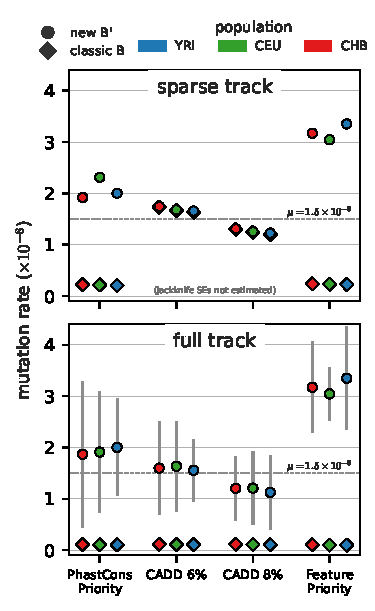
\includegraphics[width=\textwidth]{figures/figure_5.pdf} 
    \caption{(A) CADD 6\% full-track }
  \label{fig:figure-5}
\end{figure}

While we have previously shown that out-sample predicted diversity matches
observed diversity (Section XXX), we also investigated whether there were
regions of the genome that were particularly poor-fitting. Comparing predicted
against observed diversity along chromosomes (see Supplementary Materials
Section \ref{supp:chrom-fit}) we overall find close correspondence consistent
with the high $R_\text{LOCO}^2$. However, we find a few large (tens of
megabases) regions with systematically poorer fit (Supplementary Materials
Figure \ref{supp:spatial-residuals}). In Figure \ref{fig:figure-5}A we see one
such region from XXX to XXX. Interestingly, predicted diversity closely follows
the peaks and troughs of this region. We note that a smaller segment within
this region has been found by a genome-wide scan for associative overdominance
\parencite{Gilbert2020-aw}.  

Another model diagnostic is to inspect whether observations are systematically
different from predictions. We confirm the finding of \textcite{Murphy2022-sj}
that regions predicted to experience little reduction in diversity due to
background selection have higher diversity than expected (Figure
\ref{fig:figure-5}B, orange line). Their work suggested that this could reflect
ancient introgression between archaic humans and ancestors of contemporary
humans. Finally, the variance around observed and predicted diversity levels
falls very close to what we would expect under the theoretic
coalescence-noise-only expectation ($R_\text{coal}^2$).

\subsection*{Predicted Substitution Rates, and Fitness Variance}

\begin{figure}[htbp] \centering
    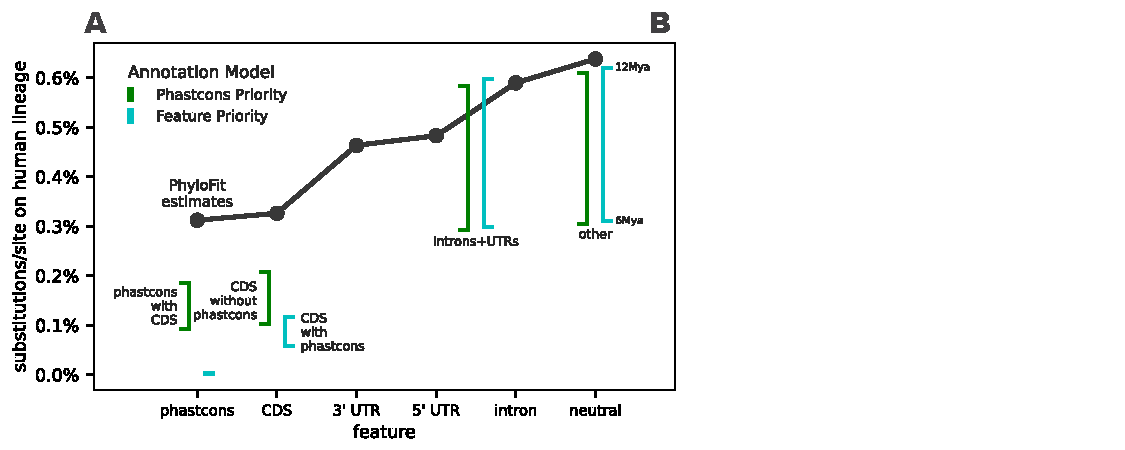
\includegraphics[width=\textwidth]{figures/figure_6.pdf} 

    \caption{Evidence that negative selection signal remains. (A) Residuals
        from the YRI CADD 6\% model plotted against the average LoF selection
        coefficient across genes in a megabase window (estimated from
        \cite{Agarwal2023-un}). Our model is systematically over predicting
        diversity in regions estimated to be sensitive to LoF variants. The
        ordinary least squares (OLS) estimate suggests that 2.1\% of the
        variance in residuals can be explained by reductions caused by the
        local sensitivity to LoF mutations. (B) Residuals from the YRI CADD 6\%
        model plotted against the fraction of CADD 6\% basepairs in the
        megabase window. Here, only 0.8\% of the variance is explained by
        remaining spatial variance in CADD 6\% regions (blue). Overlaid is the CADD
        2\% OLS curve (orange). }

  \label{fig:figure-6}
\end{figure}

Since our B' method is based upon quantitative genetic models of linked
selection that explicitly incorporates the substitution process, fitting our
model to genomic data leads to predictions that can be explicitly tested. In
particular, there are two key predicted quantities: (1) the substitution rates
per segment, and (3) the fitness variance per segment. 


Each of our maximum likelihood estimates $\widehat{\Psi}$ imply other
corresponding 



Our method accommodates weak selection by modeling the fitness variance in each
segment under an equilibrium negative selection process. This fitness variance
is found by simultaneously solving for the per-generation substitution rate $R$
and the draft-effective population size $N_d$ for each segment. When our model
is fit to genome-wide diversity data, the parameter estimates imply predictions
of the deleterious substitution rate per basepair, per generation, for each
feature. Our method only considers within-species pairwise diversity, so these
predicted substitution rates constitute a test that our model is making
reasonable out-sample predictions of the substitution rates across features.

We focus specifically on the predictions from our feature-based annotation
models, since we can readily estimate human substitution distances for each
feature to compare to our predictions.

The estimated substitution distance should in theory equal the product of the
substitution rate per site, per year and the branch length in years.

When comparing our predicted mutation rates to observed substitution distances,
we must account for three major sources of uncertainty.

First, the split time between humans and chimpanzees is unknown, with estimates
ranging from 6Mya to 12Mya (XXX). Second, our predictions are in sites per
generation, and the appropriate human generation time is unknown. Third, the
appropriate mutation rate to use is debated, since there may have been a
mutational slow down on the human lineage (XXX), which could explain why
phylogenetic- and pedigree-based mutation rate estimates differ by roughly a
factor of two (XXX). Finally, we are only considering modeling the deleterious
substitution rate. In reality, some fraction of observed substitutions fixed
because they were beneficial. 





For a particular feature $f$, the estimated per-site substitution distance
$S_f$ along a branch (which accounts for back mutations) should correspond to
$S_f = T_g r_f$, where $T_g$ is the time in generations and $r_f$ is the
substitution rate per basepair, per generation of that feature. 

Each feature is
composed of basepairs with varying selection coefficients distributed according
to the feature-specific DFE vector $\mathbf{w}_f$ and corresponding vector of
substitution rates per selection coefficient, $\mathbf{r}_f$.

Our estimate of a feature's DFE
is $\widehat{\mathbf{w}}_f$.

We calculate the 


\begin{align}
    \label{eq:sub}
    r_f = \mu \int_0^1 p_F(s) ds
\end{align}

Solving the XXX equations, we end up with predictions $\widehat{r}_f$ for the
per-basepair, per-generation substitution rate for each feature. These are
calibrated to the MLE mutation rate estimate $\widehat{\mu}_\text{del}$, which
as mentioned, excludes the contribution of lethal mutations which act purely to
reduce $N_e$ and thus only impact $\pi_0$. Using Equation \eqref{eq:sub} we can
re-calibrate these estimates against other mutation rates. 

Because of it's greater interpretabilty, we initially focus on the substitution
rate estimates from the Feature Priority model even though it had a poorer-fit
and high mutation rate estimate. 

We can also re-calibrate this model to an alternate mutation rate.

% - Table s5 https://oup.silverchair-cdn.com/oup/backfile/Content_public/Journal/genetics/206/1/10.1534_genetics.116.197145/8/files1.pdf?Expires=1686357613&Signature=cp9qoI2ChCb6GFZ74HI4eWcA~MQ4sHlWyeI3Zp49-5xEORzMfYlSRxzVvZlo8ZoGWDi0G3PnL00ZplM-~or4YIVm2uhkmqjf61AmC7RdZ1QTak4j0kFMQ0wAbM9pusiV3gIepTQHq2HKRKwgS~ypmv~0oqO5dDxaq9nhOWIBBmLAA49oHWuxUtnRe3sEYATwCwjIFEomhgJpg7vKGCF~87GdCV4JETW4PN2VvD4hsu2AVRd8yA~vUJvsXfhWwcElDeY4fsgpprl1lC3XGjJCnqdwbzRGPV5LNx5XEKLptcZtLeLcOmFJCvmVLe0bewJ7Vta0TSQM7T9AuklompjPPw__&Key-Pair-Id=APKAIE5G5CRDK6RD3PGA

Like other methods, our method divides the putatively conserved basepairs up

Generally, when the putatively conserved region is larger, there is a tradeoff
in two dimensions. First, more bases are conserved according to the same DFE,
so the total mutational load increases. This causes the tradeoff between
mutation rate estimate and CADD fraction we observe across both our B' model
and the classic B when using sparse tracks (Figure 2XXX). 


We find that mutation rate estimates are fairly sensitive to model choice
(Figure 2XXX). 

Since B' has a U-shaped relationship with the selection coefficient, we
hypothesized that our model may reveal true identifiability issues in
estimating the DFE that do not occur under the classic B model. We find that
this is not the case for our models fit at the megabase-scale. The DFE
estimates for our CADD6 and CADD8 models are consistent (Figure XXX), and both
produce similar mutation rates.

While we do not comprehensively fit all of our model to other spatial scales,
we 

However, while a given reduction level may be explained by either a weak or
strong selection coefficient, the spatial extent of these reductions caused by
weak selection is much narrower than under strong selection. 

We see evidence this is the case in several of our models, where
genome-wide diversity fits equally well between models with mutation rates 

Indeed, we see this by comparing parameter estimates of the CADD6
sparse-track model using classic BGS B and our B' method. 


(which mimics the best-fitting model of
\cite{Murphy2022-sj}) 

(see also
Appendix 1, Figure 26A of \cite{Murphy2022-sj})

correlation between s and feature

Overall, we find evidence that negative selection models are very sensitive to
the input track. Because inference based on our B' method accommodates weaker
selection, the primary models we fit here more robust to misspecification of
the regions


\section*{Discussion}

- the $pi_0$ problem

Ipsita Agarwal article 

what time scale is the average mutation being lost at?

Regularization / overfitting 

It is worth considering why this model performs well for models of negative
selection. The fitness variance equation, $V(x) = (U-2R)s$ tells us that under
models, the long-run variance is set by the balance of mutation and fixation.
Whether a particular basepair's behavior follows this equation depends upon
whether the long-run average is close to ``typical" for that basepair at a
given time. Good things fix so quickly, that we're left with a constant
churning of new variation

- need for coalescent simulations with reduced $N_e$ along the genome.

- we need to talk about Fisher's Fundamental Theorem and how this model
connects fitness variation to absolute changes in fitness.

Measuring selection in the Genome Versus Finding Selection in the Genome


\section*{Methods}
% (the method would support a new
% ``interaction" type, but this greatly increases the number of parameters).

\subsection*{Solving the B' Equations for each Segment}
\label{sec:methods-bprime-eqns}

Our software \texttt{bgspy} first calculates the equilibrium additive genic
fitness variation $\widetilde{V}_a$ and ratchet rate $\widetilde{R}$ for each
user-specified segments in the genome. These equilibria are calculated across
grids of mutation rate weighted by the DFE $m_i$ and selection coefficient
$s_j$, by numerically solving the following system of equations,

\begin{align}
  \label{eq:}
  {N}_{d} &= N \exp \left( -V_a \frac{Q^2(m_i, s_j)}{2} \right) & \text{\emph{effective population equation}} \\
  R &= \frac{4N_dU s_j}{\exp(4 N_d s_j)-1}  & \text{\emph{substitution equation}} 
\end{align}

where,

\begin{align}
  %V(x) &= U s - 2 {R}(x) s & \text{\emph{fitness variance equation}} \\
  V_a &= (U - 2 R) s_j & \text{\emph{fitness variance equation}} \\
  Q^2(m_i, s_j) &= \frac{2}{(1-Z)(2-(2-M)Z)} & \text{\emph{linkage inflation factor}} \\
  Z &= 1 - \frac{Us_j}{U-{M}} & \text{\emph{variance decay rate}}
\end{align}
%
and $U = m_i L$ and $M = r_\text{BP} L$ are the total mutation and
recombination rates in the segment. A detailed derivation of these equations
can be found in Supplementary Section \ref{supp:theory}. The recombination
rate in a segment is determined by a user-supplied recombination map.

\subsection*{Calculating the Reduction Maps}
\label{sec:methods-maps}

Our method uses the pre-computed equilibria $\widetilde{V}_{a,g}$ for each
segment $g$ to calculate the reduction map $B(x; m_i, s_j)$ at positions $x$
across the parameter grids described above. Since we assume multiplicative
fitness, the reduction is the product of each segment's contribution accounting
for the recombination is,

\begin{align}
    B(x; m_i, s_j) = \exp\left(- \frac{1}{2}\sum_{g \in G} \sum_{i=1}^{n_s} \widetilde{V}_{a,g}(m_i, s_j) Q_g^2(m_i, s_j, r_{x, g})\right)
\end{align}
%
where $r_{x, g}$ is the recombination fraction between the focal site and
segment $g$. Here, $Q^2(m_i, s_j, r_{x,g})$ is given by Equation \eqref{eq:Q}
squared. A separate reduction map is calculated for all features $G$ within a
specific feature type. We calculate B' calculate for $\log_{10}$-spaced grids
over $10^{-1} \le s \le 10^{-8}$ and $10^{-11} \le m \le 10^{-7}$, in 10kb
increments across the genome.

\subsection*{Composite Likelihood and Optimization}
\label{sec:methods-likelihood}

Following previous approaches
\parencite{McVicker2009-ax,Elyashiv2016-vt,Murphy2022-sj}, we use a composite
likelihood approach to fit our negative selection model. Per-basepair allele
count data (described below) is summarized into the number of same and
different pairwise differences per window. All of our primary models were fit
with megabase windows, since previous work has found the strongest selection
signal at this scale (we confirm this with one XXX fit at the $10^5$bp scale).

Our binomial likelihood models the number of different pairwise comparisons
observed per window given the total number of pairwise comparisons. The
binomial probability for window $b$ is $\bar{\pi}(b; \Psi) = \pi_0 \bar{B}(b;
\mu, \mathbf{W})$, where bars indicate averages over some bin width. The free
parameters $\Psi = \{\pi_0, \mu, \mathbf{W}\}$ are the expected diversity in
the absence of selection ($\pi_0$), the mutation rate ($\mu$), and the
distribution of fitness effects for the discretized selection grid and $K$
features ($\mathbf{W}$). The reduction at position $x$ is then,

\begin{align}
    \log\left(B(x; \mu, \mathbf{W}) \right) = - \frac{1}{2} \sum_{g \in G} \sum_{j=1}^{n_s} V_g(\mu W_{j, k(g)}, s_j) Q_g^2(m_i, s_j, r_{x, g}).
\end{align}
%
See Supplementary Materials Sections \ref{supp:data-summary} and
\ref{supp:likelihood} for more details.

Our method uses two tricks to improve optimization over the mutation and DFE
parameters. First, we find $B(x; \mu, \mathbf{W})$ is exponential over columns
of $\mu \mathbf{W}$, which allows for optimization over this smooth function
rather than the grid. Second, we use softmax to convert constrained
optimization over the DFE columns (which must sum to one) to unconstrained. We
tested multiple different optimization routines, finding that BOBYQA
outperformed alternatives \parencite{Powell2009-jm,Johnson2007-tl}. We
inspected and confirmed convergence with diagnostic plots finding stable optima
across 10,000 random starts (see Supplementary Materials Section
\ref{supp:optima}). We assessed model fit using out-sample predictive error,
calculated by leaving out a whole chromosome during fitting and predicting its
diversity. To calculate uncertainty, we used a block jackknife approach in 10
Mbp windows (Supplementary Section \ref{supp:jackknife}).

\subsection*{Human Population Genomic Data}
\label{sec:methods-data}

Our analyses was conducted on the Yoruba (YRI), European (CEU), and Han Chinese
(CHB) reference samples individuals from the high-coverage 1000 Human Genomes
data aligned to GRCh38/hg38 \parencite{Byrska-Bishop2022-tn}. Since nucleotide
diversity is a ratio estimator, it can be biased when subtly different
filtering criteria are applied to variant and invariant sites. To prevent this,
we conducted our analyses on Genomic VCF (gVCF) files that contain genotype
calls for both variant and invariant sites \parencite{Illumina_Inc2020-dk}.
Then, we apply the same genotype filtering criteria to all called sites
(Supplementary Materials Section \ref{supp:filter}). We also applied sequence
accessibility masks that containing only non-repeat, non-centromeric sequence
that passed the 1000 Genomes strict filter
(\cite{1000_Genomes_Project_Consortium2015-mi}; Supplementary Material Section
\ref{supp:accessible}). Since our theory only considers the indirect effects of
linked selection on a site, we additionally masked sites that are likely under
direct selective constraint (see Supplementary Materials Section
\ref{supp:neutral}). Finally, for every basepair passing these filtering and
masking criteria, we counted the number of reference and alternative allele
counts (excluding all multiallelic, indel, and CNV variants).

For all of our main analyses, we used the recombination map from
\textcite{Halldorsson2019-ey} estimated from a trio-based design to avoid
circularity that could occur by using LD-based maps. We use Ensembl gene
annotation \parencite{Cunningham2022-vk}, a special CADD Score dataset with
McVicker B scores removed (to avoid circularity;
\cite{Kircher2014-bv,Rentzsch2019-lr}), and PhastCons regions
\parencite{Siepel2005-wh}.

\subsection*{Forward Simulations}
\label{sec:methods-sim}

We conducted forward simulations of negative selection on whole human
chromosomes to validate our method at two stages. First, we simulated negative
selection on chromosome 10 using a realistic recombination map and putatively
conserved features to confirm that our classic B and new B' maps matched the
average simulation reduction map across mutation and selection parameters.
Second, we evaluated our composite likelihood method by simulating negative
selection on the first five human chromosomes, across grids of fixed mutation
and selection parameters. We then combined these into a synthetic genome, and
overlaid mutations on the ARG. Then, we ran our likelihood methods on the
resulting allele count data to assess model accuracy. We ran additional
synthetic genome simulations like these to evaluate the impact of two model
violations: recessivity of deleterious mutations and expanding populations. For
the latter, after $9.3$ generations, we grew the population by factor of 1.004
each generation to mimic the human expansion out-of-Africa
\parencite{Gutenkunst2009-pg}. We did not simulate population bottlenecks since
our analyses showed little difference between bottlenecked out-of-Africa
samples (CEU and CHB) and YRI samples. More details about these and the segment
simulations shown in Figure \ref{fig:figure-1}A-C can be found Supplementary
Section \ref{supp:simulation}.

\subsection*{Substitution Rate and Total Genic Fitness Variance Predictions}


a set of corresponding substitution rate predictions for each segment under
mutation-selection-draft process. There are two sources of variation in these
predictions in this model. First, there is the variation across the
pre-specified functional categories, e.g. CDS, UTRs, and PhastCons. Second,
there is region-specific variation 



The SC16 theory models linked selection in quantitative genetics terms and
relies on simultaneously predicting the deleterious substitution rate.

\printbibliography

\end{document}
